\documentclass[aspectratio=169]{beamer}
\usepackage[utf8]{inputenc}
\usepackage[T5]{fontenc}
\usepackage[vietnamese,english]{babel}
\usepackage{graphicx}
\usepackage{booktabs}
\usepackage{tabularx}
\usepackage{array}
\usepackage{tikz}
\usepackage{xcolor}
\usepackage{ragged2e}
\usepackage{grffile}

\usetheme{Madrid}
\usecolortheme{default}

\definecolor{smartblue}{HTML}{2563EB}
\definecolor{smartcyan}{HTML}{06B6D4}
\definecolor{smartdark}{HTML}{0F172A}
\definecolor{smartgreen}{HTML}{16A34A}

\setbeamercolor{structure}{fg=smartblue}
\setbeamercolor{frametitle}{fg=white,bg=smartblue}
\setbeamercolor{title}{fg=white,bg=smartblue}
\setbeamertemplate{navigation symbols}{}
\setbeamertemplate{itemize item}{\color{smartblue}$\blacktriangleright$}
\setbeamertemplate{itemize subitem}{\color{smartcyan}$\bullet$}

\newcolumntype{L}{>{\raggedright\arraybackslash}X}
\graphicspath{{images/}}

\title[SmartClock]{SmartClock}
\subtitle{AIoT Personal Assistant Clock}
\author{Trần Hải Đức \and Nguyễn Trọng Tài \and Nguyễn Công Chiến \and Phạm Nguyễn Gia Bảo}
\institute{Faculty of Information Technology \\ University of Science}
\date{May 26, 2026}

\begin{document}

\begin{frame}
  \titlepage
  \vspace{-0.4cm}
  \begin{center}
    \textbf{Tập trung hơn, ngủ sâu hơn, sống thông minh hơn.}
  \end{center}
\end{frame}

\begin{frame}{Agenda}
  \begin{columns}
    \column{0.48\textwidth}
    \begin{enumerate}
      \item Problem and Opportunity
      \item Product Vision
      \item Architecture and Hardware
      \item Objectives and Use Cases
    \end{enumerate}
    \column{0.48\textwidth}
    \begin{enumerate}
      \setcounter{enumi}{4}
      \item User Flow
      \item Prototype Cost
      \item Limitations
      \item Roadmap
    \end{enumerate}
  \end{columns}
\end{frame}

\begin{frame}{Problem}
  \begin{block}{Modern work and study environments are noisy}
    Người dùng dễ mất tập trung do điện thoại, mạng xã hội, thông báo và thói quen sinh hoạt thiếu ổn định.
  \end{block}
  \begin{itemize}
    \item Smartphone apps tiện lợi nhưng cũng là nguồn gây xao nhãng.
    \item Pomodoro clocks truyền thống đơn giản nhưng ít cá nhân hóa.
    \item Smartwatches nhiều tính năng nhưng chi phí cao và vẫn gây phân tâm.
    \item Người dùng cần một thiết bị nhỏ gọn, tối giản, hỗ trợ tập trung và nghỉ ngơi.
  \end{itemize}
\end{frame}

\begin{frame}{Product Vision}
  \begin{columns}
    \column{0.58\textwidth}
    \textbf{SmartClock} là thiết bị AIoT đặt trên bàn học, bàn làm việc hoặc phòng ngủ.
    \vspace{0.3cm}
    \begin{itemize}
      \item Hỗ trợ Pomodoro và luyện thuyết trình.
      \item Theo dõi giấc ngủ và đặt báo thức.
      \item Tạo trải nghiệm giải trí nhẹ bằng game và nhạc.
      \item Hoạt động cục bộ, mở rộng online qua Edge-Server.
    \end{itemize}
    \column{0.38\textwidth}
    \begin{tikzpicture}
      \draw[smartblue, line width=1.4pt, rounded corners=8pt, fill=blue!4] (0,0) rectangle (4.1,3.2);
      \node[smartblue, font=\Large\bfseries] at (2.05,2.45) {SmartClock};
      \node[align=center] at (2.05,1.55) {Focus\\Sleep\\Relax};
      \node[smartgreen, font=\small\bfseries] at (2.05,0.55) {AIoT Edge Device};
    \end{tikzpicture}
  \end{columns}
\end{frame}

\begin{frame}{Architecture}
  \begin{figure}
    \centering
    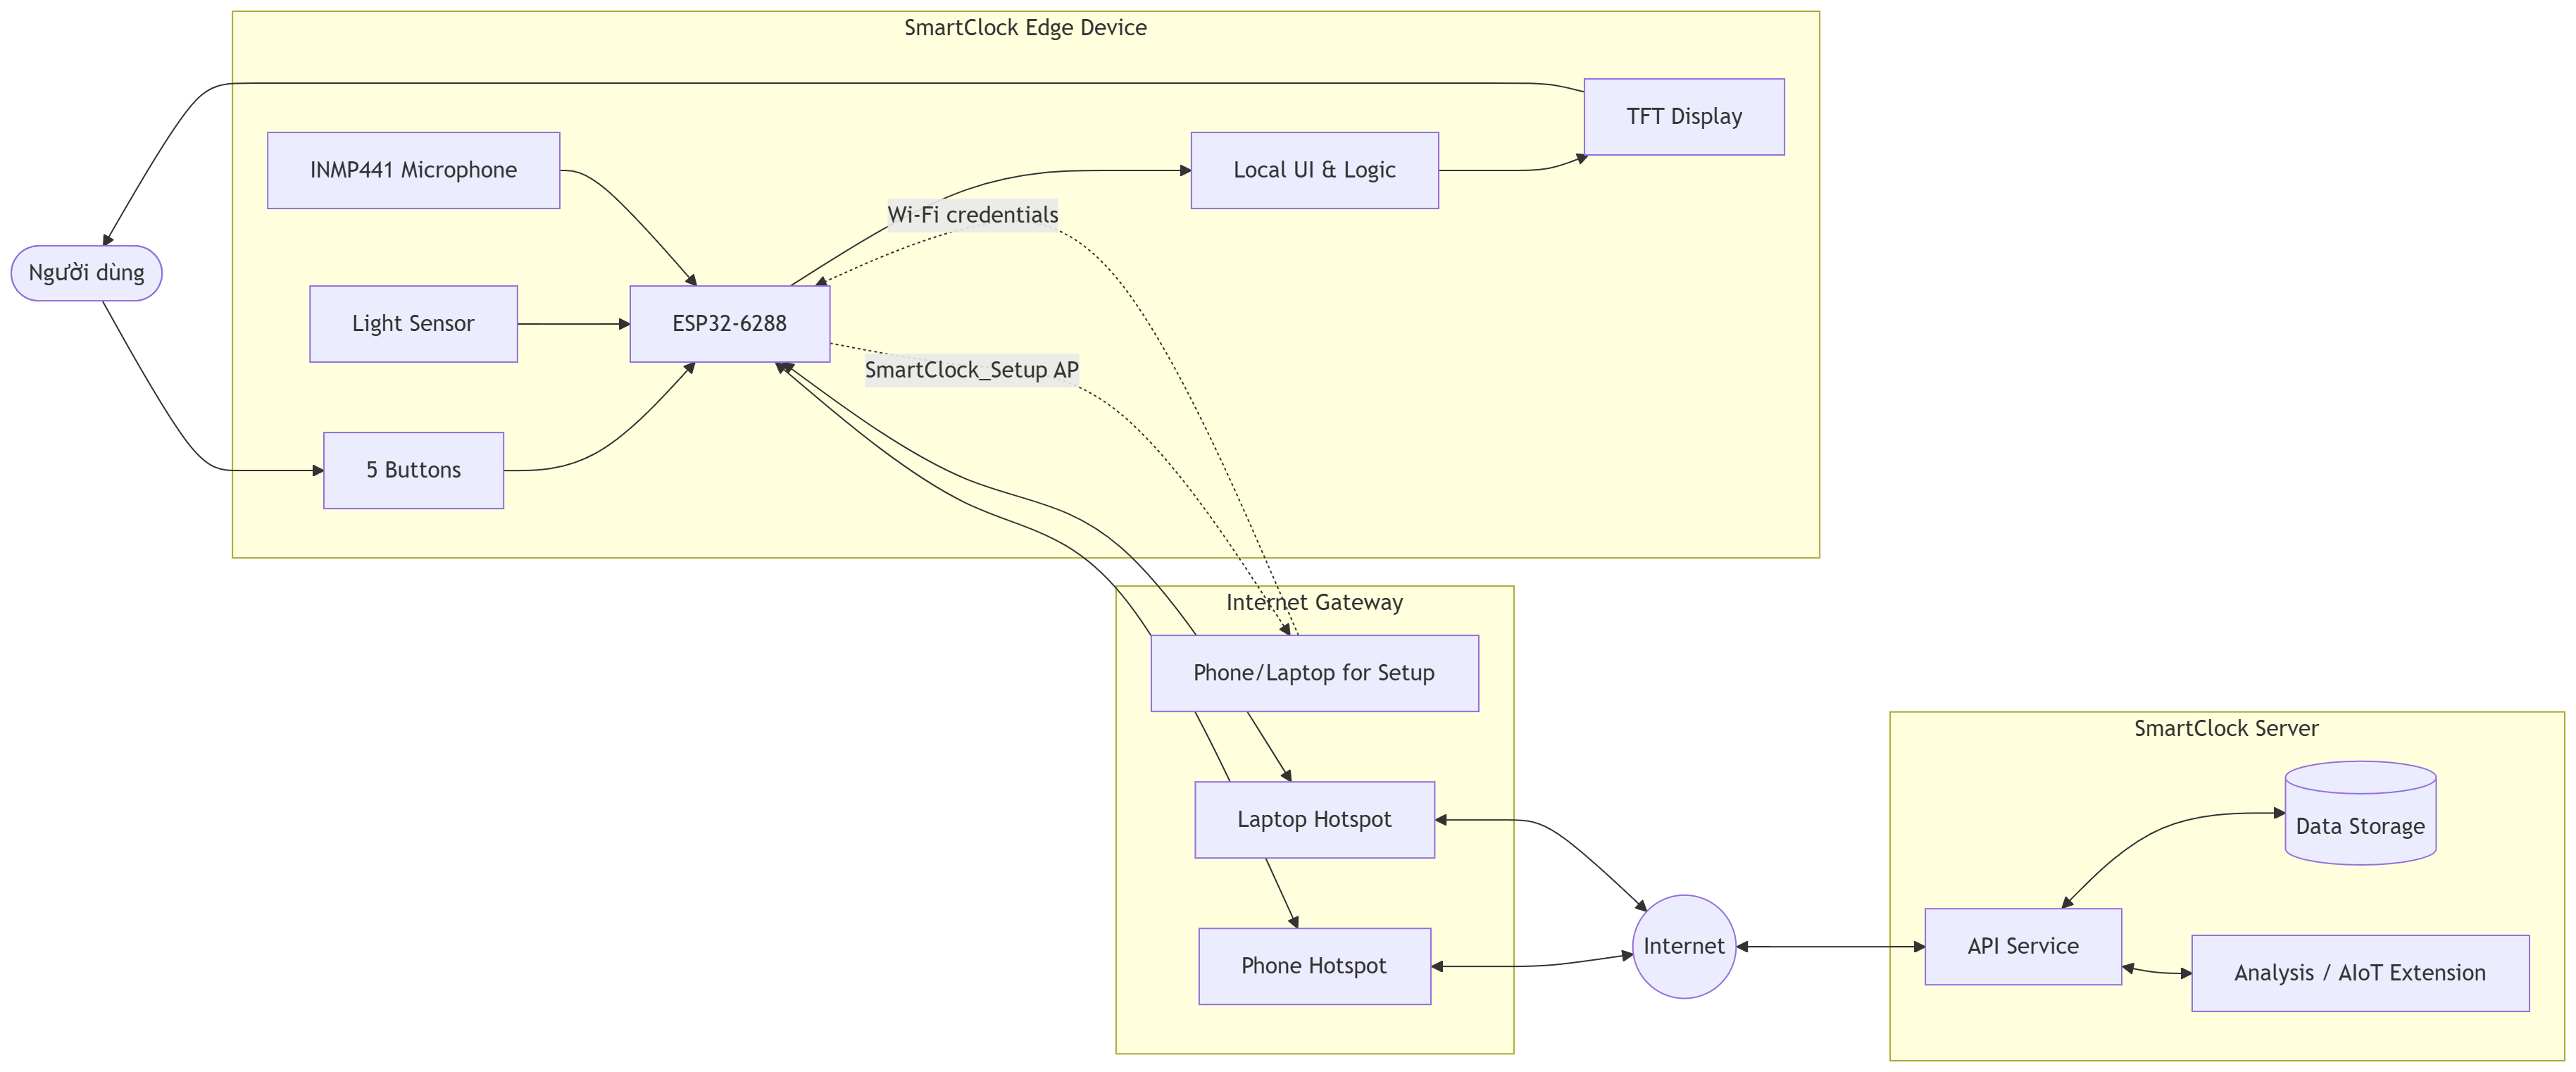
\includegraphics[width=0.86\textwidth,height=0.72\textheight,keepaspectratio]{architecture.png}
  \end{figure}
\end{frame}

\begin{frame}{Hardware Prototype}
  \small
  \begin{tabularx}{\textwidth}{@{}lLr@{}}
    \toprule
    \textbf{Component} & \textbf{Purpose} & \textbf{Estimated Price} \\
    \midrule
    ESP32-6288 & Main controller, Wi-Fi, UI logic, sensor integration & 180k--250k \\
    TFT Display & Menu, timer, sleep report, game, music UI & 120k--220k \\
    5 Buttons & Physical controls without smartphone distraction & 10k--25k \\
    Light Sensor & Environment sensing for sleep/study context & 15k--35k \\
    INMP441 & Audio sensing for ambient sound/seminar practice & 45k--80k \\
    Prototype parts & Wires, power cable, enclosure, breadboard/PCB & 115k--310k \\
    \bottomrule
  \end{tabularx}
  \vspace{0.35cm}
  \begin{block}{Estimated cost}
    Prototype cost range: \textbf{485,000 -- 920,000 VND}
  \end{block}
\end{frame}

\begin{frame}{3 Objectives}
  \begin{columns}
    \column{0.33\textwidth}
    \begin{block}{Objective 1}
      \textbf{Focus}
      \begin{itemize}
        \item Pomodoro Timer
        \item Seminar Practice
      \end{itemize}
    \end{block}
    \column{0.33\textwidth}
    \begin{block}{Objective 2}
      \textbf{Sleep}
      \begin{itemize}
        \item Sleep Monitoring
        \item Alarm Settings
      \end{itemize}
    \end{block}
    \column{0.33\textwidth}
    \begin{block}{Objective 3}
      \textbf{Relax}
      \begin{itemize}
        \item Flappy Bird
        \item Music Player
      \end{itemize}
    \end{block}
  \end{columns}
\end{frame}

\begin{frame}{Overall Use Cases}
  \begin{figure}
    \centering
    \includegraphics[width=0.82\textwidth,height=0.72\textheight,keepaspectratio]{\detokenize{UseCase (0).png}}
  \end{figure}
\end{frame}

\begin{frame}{Objective 1: Focus}
  \begin{columns}
    \column{0.48\textwidth}
    \includegraphics[width=\textwidth,height=0.56\textheight,keepaspectratio]{\detokenize{UseCase (1).png}}
    \column{0.48\textwidth}
    \begin{itemize}
      \item Pomodoro giúp chia phiên tập trung và nghỉ ngơi.
      \item Seminar Practice giúp luyện trình bày và quản lý thời lượng nói.
      \item Mục tiêu là giảm phụ thuộc điện thoại trong lúc học/làm việc.
    \end{itemize}
  \end{columns}
\end{frame}

\begin{frame}{Objective 2: Sleep}
  \begin{columns}
    \column{0.48\textwidth}
    \includegraphics[width=\textwidth,height=0.56\textheight,keepaspectratio]{\detokenize{UseCase (4).png}}
    \column{0.48\textwidth}
    \begin{itemize}
      \item Theo dõi thời gian ngủ và tạo đánh giá cơ bản.
      \item Báo thức giúp duy trì nhịp sinh hoạt ổn định.
      \item Có thể mở rộng bằng phân tích ánh sáng/âm thanh phòng ngủ.
    \end{itemize}
  \end{columns}
\end{frame}

\begin{frame}{Objective 3: Relax}
  \begin{columns}
    \column{0.48\textwidth}
    \includegraphics[width=\textwidth,height=0.56\textheight,keepaspectratio]{\detokenize{UseCase (7).png}}
    \column{0.48\textwidth}
    \begin{itemize}
      \item Flappy Bird tạo khoảng nghỉ ngắn sau phiên học/làm việc.
      \item Music Player hỗ trợ thư giãn hoặc tạo nền tập trung.
      \item Tăng tính gần gũi và thẩm mỹ cho góc làm việc.
    \end{itemize}
  \end{columns}
\end{frame}

\begin{frame}{User Flow}
  \begin{center}
    \Large
    \texttt{HOME} $\rightarrow$ \texttt{STUDY} $\rightarrow$ \texttt{SLEEP} $\rightarrow$ \texttt{RELAX} $\rightarrow$ \texttt{HOME}
  \end{center}
  \vspace{0.4cm}
  \begin{itemize}
    \item One physical Mode button cycles through main modes.
    \item Remaining buttons perform context actions.
    \item Internet setup: \texttt{SmartClock\_Setup AP} then phone/laptop hotspot.
    \item Offline mode still supports core local functions.
  \end{itemize}
\end{frame}

\begin{frame}{Business Value}
  \begin{itemize}
    \item \textbf{Productivity:} helps students and knowledge workers build focus routines.
    \item \textbf{Wellness:} encourages consistent sleep and wake-up habits.
    \item \textbf{Affordability:} prototype uses low-cost, accessible components.
    \item \textbf{Expansion:} Edge-Server architecture supports analytics and personalization later.
  \end{itemize}
\end{frame}

\begin{frame}{Limitations and Roadmap}
  \begin{columns}
    \column{0.48\textwidth}
    \textbf{Limitations}
    \begin{itemize}
      \item Sleep and seminar evaluation are basic.
      \item Hardware cost is prototype-level estimation.
      \item Wi-Fi setup needs secure UX.
    \end{itemize}
    \column{0.48\textwidth}
    \textbf{Roadmap}
    \begin{itemize}
      \item Better enclosure and PCB.
      \item History dashboard.
      \item Personalized schedules.
      \item Smart Home / AIoT integration.
    \end{itemize}
  \end{columns}
\end{frame}

\begin{frame}
  \begin{center}
    \Huge Thank You
    \vspace{0.6cm}

    \Large SmartClock
    \vspace{0.2cm}

    \normalsize Tập trung hơn, ngủ sâu hơn, sống thông minh hơn.
  \end{center}
\end{frame}

\end{document}
